\subsection{Dimension Reduction}
Dimension reduction incorporates a broad class of techniques used for visualizing high-dimensional datasets, but in some cases can be useful for parameter screening.
%
Dimension reduction techniques can be roughly divided into two major categories: linear dimension reduction and nonlinear dimension reduction (manifold learning).
%%Are manifold learning methods able to be used for parameter screening? I don't think so because they lose intuition in the original space.

\subsubsection{Linear Projection.}
Linear projection uses a linear transformation to project the data from high-dimensional to low-dimensional space.
%
The methods here vary only in how they optimize the linear projection of the data and include such classical methods as Principal Component Analysis (PCA), Multidimensional Scaling (MDS), Linear Discriminant Analysis (LDA), and the various factor analysis methods.

PCA~\cite{Jolliffe2005} is designed to find an orthogonal linear transformation that maximizes the variance of the resulting embedding.
%
PCA can be calculated by an eigen decomposition of the data's covariance matrix or a singular value decomposition of the data matrix.
%
Interactive PCA (iPCA)~\cite{JeongZiemkiewiczFisher2009} visualizes the results of PCA using multiple coordinated views.
%
The system allows synchronized exploration and manipulations among the original data space, the eigenspace, and the projected space, which aids the user in understanding both the PCA process and the dataset.
%
When visualizing labeled data, class separation is usually desired.
%
Methods such as LDA aim to provide a linear projection that maximizes the class separation.
%
The work by Koren et al.~\cite{KorenCarmel2003} generalizes PCA and LDA by providing a family of flexible linear projections to cope with different kinds of data.

\subsubsection{Nonlinear Dimension Reduction.}
Nonlinear dimension reduction can occur in  either a metric or nonmetric setting.
%
The graph-based techniques are designed to handle \textit{metric} inputs, such as Isomap~\cite{TenenbaumSilvaLangford2000}, Locally Linear Embedding (LLE)~\cite{RoweisSaul2000}, and Laplacian Eigenmap (LE)~\cite{BelkinNiyogi2003}, where a neighborhood graph is used to capture local distance proximities and build a data-driven model of the space.
%
% Isomap is one of such example.
% %
% As mentioned previously, Isomap is essentially a metric MDS where the Euclidean distance is replaced by the Geodesic distance calculated on the manifold.
% %
% The Geodesic distance is approximated by calculating the shortest path on the neighborhood graph, which itself is an approximation of the underlying manifold structure.
% %
% Other graph based manifold learning methods following a divide and conquer approach.
% %
% The representatives of these methods are the Local Linear Embedding(LLE)~\cite{roweis2000nonlinear} and Laplacian Eigenmap~\cite{belkin2003laplacian}.
% %
% The LLE models the manifold by represents each point as a weighted linear combination of its neighbors and tries to preserve this linear relationship in the reduced dimensional space.
% %
% The Laplacian Eigenmap~\cite{belkin2003laplacian} attempts to capture the neighboring information through the use of the graph laplacian.
% %
% The final embedding is calculated by an Eigen decomposition of the graph laplacian matrix.
%
These methods generate a low-dimensional nonlinear embedding that preserves local information along the manifold.
%
However, compared to the linear projections, the nonlinear embedding is much harder to interpret, and the out-of-sample points cannot be easily projected into the same domain.
%
In addition, each of these methods has certain parameters we need to tune in order to obtain a desirable result for different data and applications.
%
These limited their effectiveness as visualization tools for high-dimensional dataset.
%
Moreover, the graph-based methods are very sensitive to the construction process of the underlying neighborhood graph.
%
% In Isomap, for example, changing the number of neighbors in the graph may lead to drastic changes in the final nonlinear embedding.
%
Besides graph-based methods, various applications require the display of nonmetric dissimilarities.
%
The methods addressing the nonmetric problem are stress-based manifold learning methods, also referred as nonmetric MDS or stress-based MDS.

The stress is defined as follow.
%
Let $d_{ij}$ be the distance between a pair of points $i, j$ in $\mathbb{R}^l$ and $\hat{d}_{ij}$ be the corresponding distance in $\mathbb{R}^m$. Then the stress is defined as, $ S = \frac{\sum_{i,j}(d_{ij}-\hat{d}_{ij})^2}{\sum_{i,j}d_{ij}^2}.$
%
The other group of techniques addresses nonmetric problems commonly referred to as nonmetric MDS or stress-based MDS by capturing nonmetric dissimilarities.
%
The fundamental idea behind the nonmetric MDS is to minimize the mapping error directly through iterative optimizations.
%
The well-known Shepard-Kruskal algorithm~\cite{Kruskal1964} begins by finding a monotonic transformation that maps the nonmetric dissimilarities to the metric distances, which preserves the rank-order of dissimilarity.
%
Then, the resulting embedding is iteratively improved based on stress.
%
The progressive and iterative nature of these methods has been exploited recently by Williams et al.~\cite{WilliamsMunzner2004}, where the user is presented with a coarse approximation from partial data.
%
The refinement is on-demand based on user inputs.
%
Others rely on hybrid methods~\cite{MorrisonRossChalmers2002, MorrisonChalmers2003} based upon stochastic sampling and interpolation to approximate the solution.

t-SNE~\cite{MaatenHinton2008} has gained a lot of attention recently due to its effectiveness for visualizing high-dimensional data.
%
It utilizes a probability distribution to encode the inter-point neighborhood information, and a mismatched distribution between high- and low-dimensional spaces is used to eliminate the unwanted attractive forces, therefore, resolving the crowding problem~\cite{MaatenHinton2008}.

\begin{figure}[!ht]
  \centering
  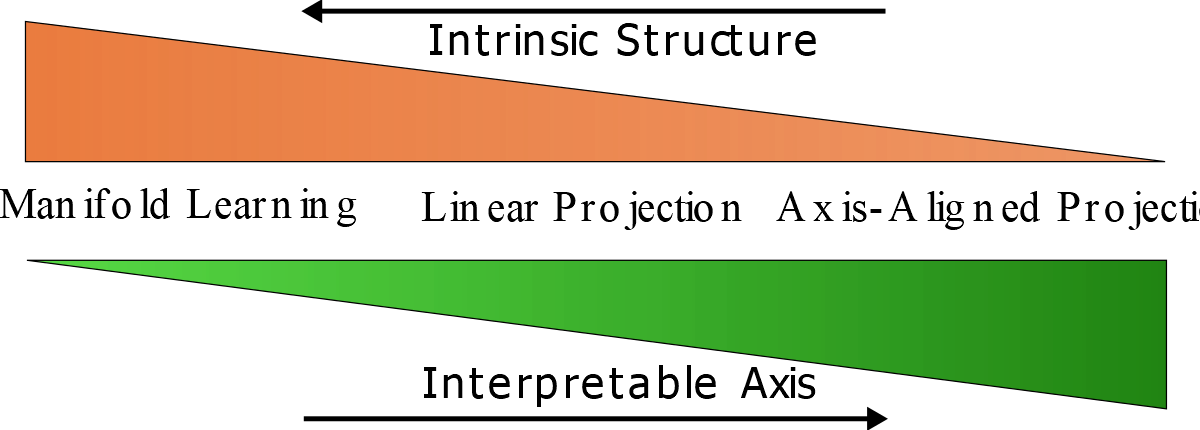
\includegraphics[width=0.47\textwidth]{interpretableAxis}
  \vspace{-2mm}
  \caption{A trade-off exists between the interpretablility of the axis and the intrinsic structure captured by the dimensionality reduction methods.}
  \label{fig:tradeOffProjections}
\end{figure}

The trade-off among the different type of projections is illustrated in Fig.~\ref{fig:tradeOffProjections}.
%
The bivariate scatterplot (as in a scatterplot matrix) is most easily understood, since its axes directly correspond to the original dimensions.
%
A linear projection~\cite{KorenCarmel2003,Jolliffe2005} generates interpretable embeddings (less so compared to a bivariate scatterplot),
and the out-of-samples points can be easily projected to the same space.
%
The non-linear projection (manifold learning) approaches~\cite{TenenbaumSilvaLangford2000, RoweisSaul2000, BelkinNiyogi2003},
on the other hand, allow the capture of more complex structures, but the resulting embedding can be extremely difficult to interpret.
%

\subsubsection{Control Point Based Projection.}
For handling large and complex datasets, the traditional linear or nonlinear dimension reductions are limited by their computational efficiency.
%
Some recent developments, e.g.,~\cite{SilvaTenenbaum2004, PaulovichSilvaNonato2010, PaulovichElerPoco2011}, utilize a two-phase approach, where a set of control points (or anchor points) is projected first, followed by the projection of the rest of the points based on the location of the control points and preservation of local features.

Such designs lead to a much more scalable system.
%
Furthermore, the control points allow the user to easily manipulate and modify the outcome of the dimension reduction computation to achieve the desired results.

\subsubsection{Distance Metric.}
For a given dimension reduction algorithm, a suitable distance metric is essential for the computation outcome as it is more likely to reveal important structural information.
Brown et al.~\cite{BrownLiuBrodley2012} introduce the distance function learning concept, where a new distance metric is calculated from the manipulation of point layouts by an expert user.
In the \emph{Explainers} work~\cite{Gleicher2013}, the author attempts to associate a linear basis with a certain meaningful concept constructed based on user-defined examples. Machine learning techniques can then be employed to find a set of simple linear bases that achieve an accurate projection according to the prior examples.
The structure-based analysis method~\cite{LeeMcDonnellZelenyuk2014} introduces a data-driven distance metric inspired by the perceptual processes of identifying distance relationships in parallel coordinates using polylines.

\subsubsection{Dimension Reduction Precision Measure.}
One of the fundamental challenges in dimension reduction is assessing and measuring the quality of the resulting embeddings.
Lee et al. introduce the ranking-based metric~\cite{LeeVerleysen2009} that assesses the ranking discrepancy before and after applying dimension reduction.
This technique is then generalized~\cite{MokbelLueksGisbrecht2013} and used for visualizing dimension reduction quality.

A projection precision measure is introduced in~\cite{SchreckLandesbergerBremm2010}, where a local precision score is calculated for each point with a certain neighborhood size.
In the distortion-guided exploration work~\cite{LiuWangBremer2014}, several distortion measures are proposed for different dimension reduction techniques, for which these measures aid in understanding the cause of highly distorted areas during interactive manipulation and exploration.
For MDS, the stress can be used as a precision measure. Seifert et al.~\cite{SeifertSabolKienreich2010} further develop this idea by incorporating the analysis and visualization for better understanding of the localized stress phenomena.
%\SL{
In recent work~\cite{StahnkeDorkMuller2016}, Stahnke et al. introduce the notion of probing for examining the dimension reduction results. This approach not only reveals  points with larger errors but also interactively considers locally correct representations of these points.
%}

\subsection{Subspace Clustering}
\label{sec_subspace}
Clustering is one of the most widely used data-driven analysis methods.
%
Instead of providing an in-depth discussion of all clustering techniques, in this survey we focus on subspace clustering techniques that have a great impact on understanding and visualizing high-dimensional datasets.
%
Compared to dimension reduction, which aims to compute one single embedding that best describes the structure of the data, subspace clustering helps identify multiple embeddings, each capturing a different aspect of the data, by clustering either the dimensions or the data points.

\subsubsection{Dimension Space Exploration.}
Guided by the user, dimension space exploration methods interactively group relevant dimensions into subsets.
%
The grouping allows us to better understand dimension relationships and to identify shared patterns among the dimensions.
%
Turkay et al. introduce a \emph{dual} visual analysis model~\cite{TurkayFilzmoserHauser2011} where both the dimension embedding and point embedding can be explored simultaneously.
%
Their later improvement~\cite{TurkayLundervoldLundervold2012} allows for the grouping of a collection of dimensions as a \emph{factor}, which permits effective exploration of the heterogeneous relationships among them.
%
The Projection Matrix/Tree work~\cite{YuanRenWang2013} extends a similar concept to allow a recursive exploration of both the dimension space and data space.
%
One recent advance~\cite{ChengMueller2016} bridges the gap between the dimension space and the data space.
%
By combining the dimension and element relationship and encoding them into a single matrix, the proposed approach produces a comprehensive map in which the data points are presented in the context of the variables.


\subsubsection{Subsets of Dimensions.}
Compared to the dimension space exploration, where the user is responsible for identifying patterns and relationships, subspace clustering/finding methods automatically group related dimensions into clusters.
%
Subspace clustering filters out the interferences introduced by irrelevant dimensions, allowing lower-dimensional structures to be discovered.
%
These methods, such as ENCLUS~\cite{ChengFuZhang1999}, originate from the data mining and knowledge discovery community.
%
They introduce some very interesting exploration strategies for high-dimensional datasets that can be particularly effective when the dimensions are not tightly coupled.
%
The $TripAdvisor^{ND}$~\cite{NamMueller2013} system employs a sightseeing metaphor for high-dimensional space navigation and exploration.
%
It utilizes subspace clustering to identify the sights for the exploration.
%
The subspace search and visualization work~\cite{TatuMaabFarber2012} utilizes the SURFING~\cite{BaumgartnerPlantRailing2004} algorithm to search the high-dimensional space and automatically identifies a large candidate set of interesting subspaces.
%
In the work presented by Ferdosi et al.~\cite{FerdosiBuddelmeijerTrager2010}, morphological operators are applied on the density field generated from the (3D) PCA projection of the high-dimensional data for identifying subspace clusters.

\subsubsection{Non-Axis-Aligned Subspaces.}
Instead of grouping the dimensions, which essentially creates axis-aligned linear subspaces, identifying non-axis-aligned linear subspaces is a more flexible alternative.
%
Projection Pursuit~\cite{FriedmanTukey1974} is one of the earliest works aimed at automatically identifying the interesting non-axis-aligned subspaces, where the projections are considered to be more interesting when they deviate more from a normal distribution.
%
Recently, some advances have been made in the machine learning community to perform non-axis-aligned subspace clustering~\cite{Vidal2011}.
%
Instead of finding (possibly overlapping) clusters in axis-aligned subspaces defined by different dimensions combinations, the points are directly clustered together for sharing similar linear subspaces.
%
In particular, this approach assumes the complex structure of the data can be approximated by a mixture of linear subspaces (of varying dimensions), and each of the linear subspaces corresponds to a set of points where their relationships can be approximately captured by the same linear subspace.
%
Lehmann et al. ~\cite{LehmannTheisel2016} have recently introduced an interesting and different approach for identifying a set of distinct linear projections.
%
By adopting a dissimilarity measure, they aim to remove duplicated data patterns by optimizing the dissimilarity among the selected projections.
%
By utilizing random projection~\cite{BinghamMannila2001}, Anand et al.~\cite{AnandWilkinsonDang2012} introduce an efficient subspace finding algorithm for data with thousands of dimensions.
%
The algorithm generates a set of candidate subspaces through random projections and presents the top-scoring subspaces in an exploration tool.